\section{Modeling}
\label{sec:modeling}


% %
% SYSTEM DESCRIPTION
% %
We consider the system depicted in Figure \ref{fig:modeling-system-sketch}, consisting of:

\begin{itemize}
	\item  mobile devices sending tasks partitioned in two classes, whose arrival process is exponential with rates $\lambda_{i}$;
	\item a Cloudlet with $N$ servants, whose service process is exponential with rate  $\mu_{clt,i}$;
	\item a remote Cloud server with virtually unlimited resources, whose service process is exponential with rate  $\mu_{cld,i}$;
	\item a front-dispatcher, responsible to route requests to Cloudlet or Cloud, according to the policy defined in Algorithm \ref{alg:modeling-dispatching-policy}, that takes into account the number $n_{clt}$ of tasks in Cloudlet, the number $n_{cld}$ of tasks in Cloud and the threshold $S$.
\end{itemize}

\begin{figure}
	\label{fig:modeling-system-sketch}
	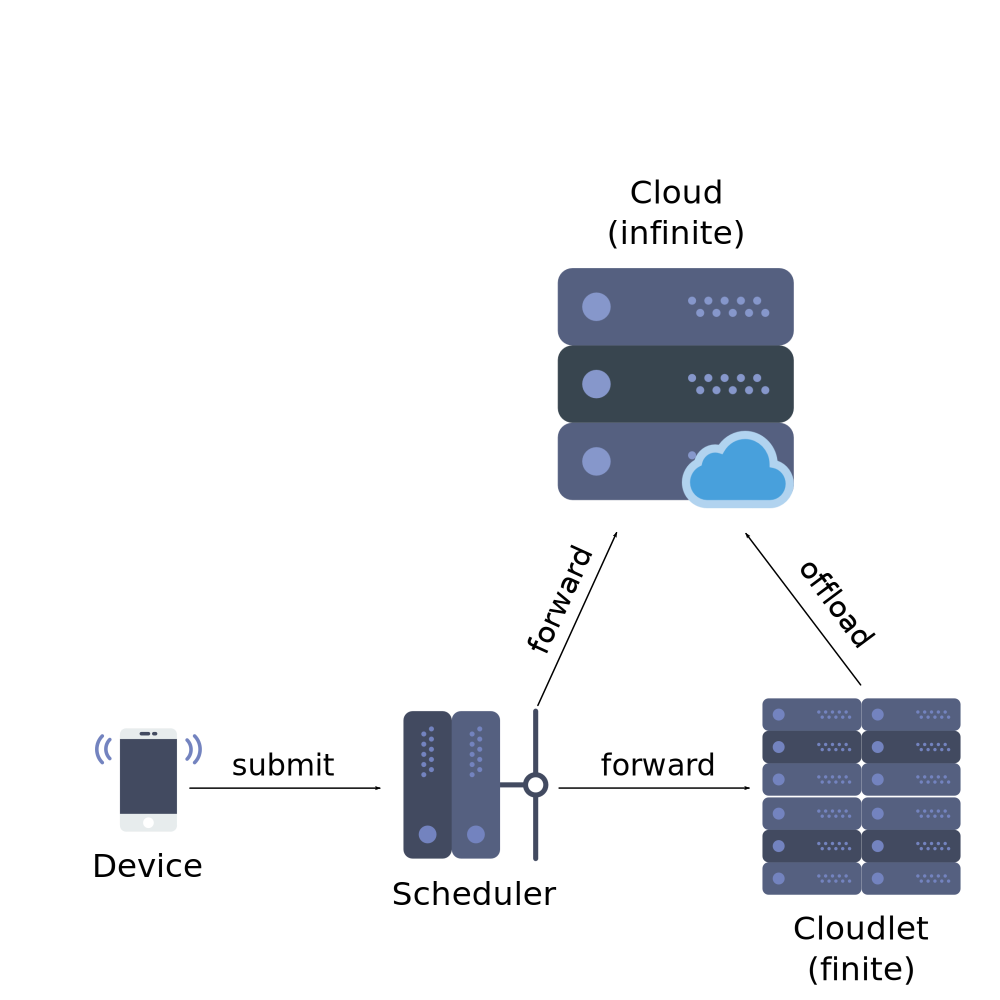
\includegraphics[width=\columnwidth]{fig/modeling-system-sketch}
	\caption{The system sketch.}
\end{figure}

We assume that service time includes the transmission time and $\mu_{clt,i}>\mu_{cld,i}\ \forall i=1,2$.
When a class 2 task is interrupted in the Cloudlet and sent to the cloud, an exponentially distributed setup time $T_{setup}$ has to be considered to restart the task on the Cloud.

\begin{algorithm}
	\label{alg:modeling-dispatching-policy}
	\SetAlgoLined
	\If{$arrival\in C_{1}$}{
		\If{$n_{1}=N$}{
			send on the cloud
		} 
		\If{$n_{1}+n_{2}<S$}{
			accept
		} 
		\eIf{$n_{2} > 0$}{
			accept the task on the cloudlet and send a class 2 task on the cloud
		}{
			accept the task on the cloudlet
		}
	}
	\If{$arrival\in C_{2}$}{
		\eIf{$n_{1}+n_{2}>=S$}{
			send on the cloud
		}{
			accept the task on the cloudlet
		}
	}
	\caption{The dispatching policy.}
\end{algorithm}


% %
% GOALS AND OBJECTIVES
% %
The main goal of the simulation is to determine with a $95\%$ level of confidence
(i) the response time and the throughput as a function of the threshold $S$
(ii) the distribution of the response time when $S=N$ and
(iii) the threshold $S*$ that minimizes the response time.


% %
% CONCEPTUAL MODEL
% %
The conceptual model is depicted in Figure \ref{fig:modeling-conceptual-model}.

\begin{figure}
  \label{fig:modeling-conceptual-model}
  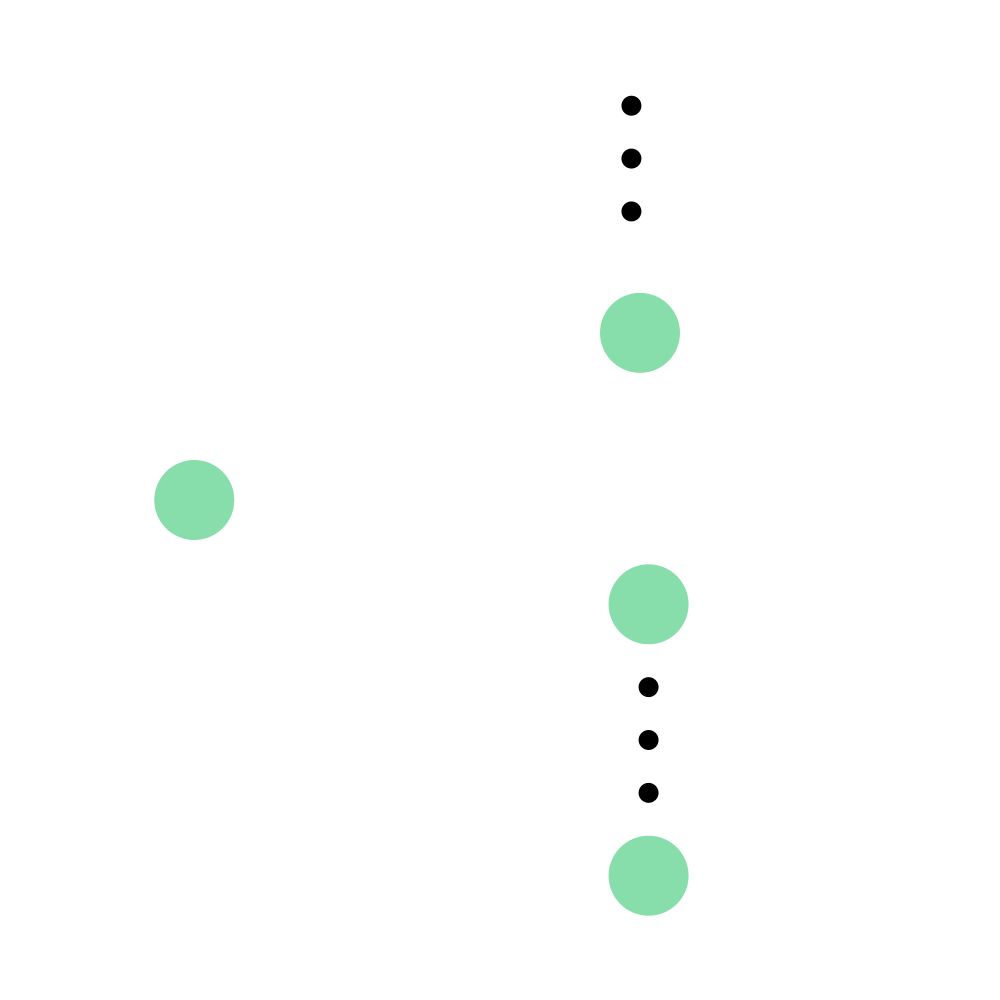
\includegraphics[width=\columnwidth]{fig/modeling-conceptual-model}
  \caption{The conceptual model.}
\end{figure}

% %
% SPECIFICATION MODEL
% %
The state of the system is represented by the pair $(n_{1},n_{2})$, where $n_{1}$ is the number of tasks in Cloudlet and $n_{2}$ is the number of tasks in Cloud.

% %
% VERIFICATION
% %
The model has been verified by ... 

% %
% VALIDATION
% %
It is well-known that model development includes a final validation step. Clearly, we cannot conduct such a final process because we cannot compare model results with a real system.